\section{Tracer une fonction}

Lua détermine les points nécessaires pour tracer la courbe. Le nombre de points est fixé par l'option \tkzname{samples}. \TIKZ\ trace ensuite la ligne qui joint ces points.

\subsection{Définir une fonction : \tkzcname{tkzFnDef}}

\begin{NewMacroBox}{tkzFnDef}{\marg{nom}\marg{expression}}
\emph{Définit une fonction de la variable \texttt{x}. Le nom est un nom Lua (lettres, chiffres, \texttt{\_}). La fonction est ensuite désignée par son nom dans toutes les macros : \tkzcname{tkzFnDraw}\texttt{(f)}, \tkzcname{tkzFnTangent}\texttt{(f,1)}, \tkzcname{tkzFnArea}\texttt{(f)}, etc. En Lua, elle est rangée dans la table \texttt{FN} : \texttt{FN.f(2)}.}

\begin{tabular}{lll}
\toprule
arguments             & exemple & explication  \\
\midrule
\TAline{nom}{f}{nom de la fonction}
\TAline{expression}{x\string^3-2*x}{expression Lua en x}
\bottomrule
\end{tabular}
\end{NewMacroBox}

\subsection{Tracer une fonction : \tkzcname{tkzFnDraw}}

\begin{NewMacroBox}{tkzFnDraw}{\oarg{options}\parg{nom} \textrm{ou} \oarg{options}\marg{expression}}
\emph{La fonction est désignée par son nom, ou bien donnée directement par son expression ; l'option \tkzname{name} permet alors de lui donner un nom.}

\begin{tabular}{lll}
\toprule
options             & défaut & définition     \\
\midrule
\TOline{domain}{xmin:xmax}{domaine du tracé}
\TOline{samples}{200}{nombre de points calculés}
\TOline{name}{}{nom donné à la fonction}
\TOline{clip}{true}{la courbe est découpée à la fenêtre}
\TOline{mark=\dots}{}{marque en chaque point calculé (\tkzname{plotmarks})}
\TOline{smooth}{}{courbe lissée par \TIKZ}
\bottomrule
\end{tabular}

\emph{Les autres options sont celles de \TIKZ ; le style est \tkzname{tkzfn curve}.}
\end{NewMacroBox}

\tkzHand Il faut avoir initialisé le repère à l'aide de \tkzcname{tkzFnInit} avant d'appeler \tkzcname{tkzFnDraw}.

\tkzHand La courbe est interrompue là où la fonction n'est pas définie (|ln(x)| pour $x\leq 0$) et lorsqu'elle passe d'un bord de la fenêtre à l'autre (asymptote verticale).

%<--------------------------------------------------------------------------->
\subsection{Option : \tkzname{samples}}

Pour tracer une droite, deux points suffisent : \tkzname{samples=2}. On demande ici 400 points ; par défaut, la valeur choisie est 200.

\begin{tkzexample}[latex=7cm]
\begin{tikzpicture}[scale=1]
    \tkzFnInit[xmin=0,xmax=5,
               ymin=0,ymax=2]
    \tkzFnGrid[sub]
    \tkzFnAxes
    \tkzFnDraw[samples=400,
               domain=.5:5]{1/x}
\end{tikzpicture}
\end{tkzexample}

%<--------------------------------------------------------------------------->
\subsection{Options : \tkzname{xstep, ystep}}

\begin{tkzexample}[]
\begin{tikzpicture}
\tkzFnInit[xmin=0,xmax=110,xstep=10,
           ymin=0,ymax=6,ystep=1]
\tkzFnAxisX[label={\textit{Âge}},
            label style={below=12pt,left}]
\tkzFnAxisY[label={\textit{Litres}}]
\tkzFnDraw[domain=0.1:100]{50/x}
\end{tikzpicture}
\end{tkzexample}

\subsection{Modification de \tkzname{xstep} et \tkzname{ystep}}

Cette fois le domaine s'étend de 0 à 700 et les valeurs prises par la fonction de $0$ à $\tkzFnPrint{1200}$. Avec \tkzname{tkz-fct}, il fallait écrire |\x| à la place de $x$ et |1./90000| à la place de |1/90000| ; ce n'est plus nécessaire.

\begin{tkzexample}[vbox]
\begin{tikzpicture}[scale=1.5]
 \tkzFnInit[xmin=0,xmax=700,xstep=100,
            ymin=0,ymax=1200,ystep=400]
 \tkzFnGrid(0,0)(700,1200)  \tkzFnAxes
 \tkzFnDraw[color=red,samples=100,line width=0.8pt,domain=0:700]
        {(1/90000)*x^3-(1/100)*x^2+(113/36)*x}
\end{tikzpicture}
\end{tkzexample}

\subsection{\tkzname{ystep} et les fonctions constantes}

Avec \tkzname{gnuplot}, |80/6| était une division euclidienne et il fallait écrire |80.| ; avec Lua, les calculs sont toujours faits sur des nombres décimaux.

\begin{tkzexample}[vbox]
 \begin{tikzpicture}[scale=0.4]
 \tkzFnInit[xmin=0,xmax=30,ymin=0,ymax=90,ystep=6]
 \tkzFnAxisX[ticks=false,label=$t$]
 \tkzFnAxisY[ticks=false,label=$P$]
 \tkzFnDraw[line width=1pt,color=red,dashed,domain=0:30]{80}
 \tkzFnDraw[line width=1pt,color=blue,domain=0:30]{80/(1+4*exp(-0.21*x))}
 \tkzFnText[above,color=red](20,80){$P=80$}
\end{tikzpicture}
\end{tkzexample}

\subsection{Les fonctions affines ou linéaires}
Pour obtenir une droite, deux points suffisent : \tkzname{samples=2}.

\begin{tkzexample}[vbox]
 \begin{tikzpicture}[]
 \tkzFnInit[xmin=0,xmax=10,ymin=0,ymax=20,ystep=5]
 \tkzFnAxes
 \tkzFnDraw[color=red,domain=0:10,samples=2]{2*x+5}
 \tkzFnDraw[color=blue,domain=0:10,samples=2]{-x+15}
 \tkzFnDraw[color=green,domain=0:10,samples=2]{7}
\end{tikzpicture}
\end{tkzexample}

%<--------------------------------------------------------------------------->
\subsection{Sous-grille}

   $y=(x-4)\text{e}^{-0.25x+5}$

Il est possible de dessiner une autre grille sur une partie du repère (voir aussi la section précédente).

\begin{tkzexample}[latex=8cm]
\begin{tikzpicture}[scale=.8]
 \tkzFnInit[xmin=4,xmax=18,xstep=2,
            ymin=20,ymax=90,ystep=10]
 \tkzFnDraw[domain=5:18]
        {(x-4)*exp(-0.25*x+5)}
 \tkzFnGrid(4,20)(18,90)
 \tkzFnAxes
 \tkzFnGrid[sub,
            subdx=0.5,
            subdy=2,
            color=brown](6,60)(12,90)
\end{tikzpicture}
\end{tkzexample}

%<--------------------------------------------------------------------------->
\subsection{Textes et points}

\begin{center}
\begin{tkzexample}[vbox]
\begin{tikzpicture}[scale=2]
 \tkzFnInit[xmin=-3,xmax=3,ymin=-1,ymax=4]
 \tkzFnGrid[sub,subdx=.5,subdy=.5]
 \tkzFnAxes
 \tkzFnDraw[domain=-3:2]{(2-x)*exp(x)}
 \tkzFnText(-2,1.25){$\mathcal{C}_{f}$}
 \tkzFnDefPointXY[draw](2,0){A}
 \tkzFnLabelPoints(A)
\end{tikzpicture}
\end{tkzexample}
\end{center}

\endinput
